\begin{figure}[ht]
 \centering
 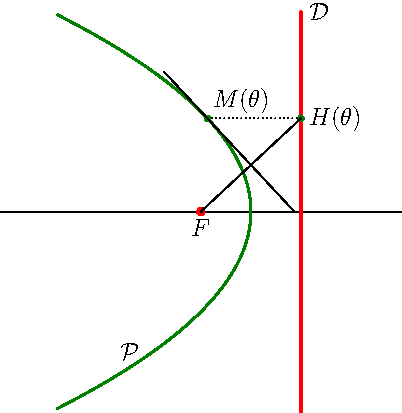
\includegraphics[width=5cm]{Eco03_1.pdf}
 % Eco03_1.pdf: 142x4 px, 72dpi, 5.01x0.14 cm, bb=0 0 142 4
 \caption{Exercice \arabic{enumi} : tangente à une parabole}
 \label{fig:Eco3_1}
\end{figure}

\begin{tiny}(Eco03)\end{tiny} Propriétés des tangentes : parabole.\newline
Dans un plan muni d'un repère orthonormé, on se donne un réel $p>0$, un point $F$ et une parabole $\mathcal P$ paramétrée par :
\begin{displaymath}
 M(\theta) = F + \frac{p}{1+ \cos\theta}\overrightarrow{e_\theta}.
\end{displaymath}
Déterminer des expressions simples de $\lambda(\theta)$ et $\varphi(\theta)$ pour que
\begin{displaymath}
 \overrightarrow{M'}(\theta) = \lambda(\theta)\overrightarrow{e_{\varphi(\theta)}}.
\end{displaymath}
En déduire que la tangente (figure \ref{fig:Eco3_1}) est la médiatrice de $FH(\theta)$. Comment se réfléchit sur $\mathcal P$ un rayon parallèle à l'axe focal ?
